% This is LLNCS.DEM the demonstration file of
% the LaTeX macro package from Springer-Verlag
% for Lecture Notes in Computer Science,
% version 2.4 for LaTeX2e as of 16. April 2010
%
\documentclass{llncs}
\usepackage{epsfig,graphicx,natbib}
%
\usepackage{makeidx}  % allows for indexgeneration
%
\begin{document}
%

\mainmatter              % start of the contributions
%
%% Ubiquitous Assistant
%% Ambient Assistance
%% Star Trek
%% Persistent Assistant
%% First-Person Multi-modal

%% Building a Ubiquitous Assistant with Multi-Modal First-Person Sensing
%% Enhancing

%% Interacting with Environment
%% Query the Environment

%% Information Retrieval 

%% MMFPQ
%% Multi-Modal First-Person Querying
\title{\large Multi-Modal First-Person Querying}
%\title{Multimodal First-Person Querying}
%
\titlerunning{Collaborative Querying with MMFPS}  % abbreviated title (for running head)
%                                     also used for the TOC unless
%                                     \toctitle is used
%
\author{
Anonymous
%Ivar Ekeland\inst{1} \and Roger Temam\inst{2}
%Jeffrey Dean \and David Grove \and Craig Chambers \and Kim~B.~Bruce \and
%Elsa Bertino}
%
\authorrunning{Anonymous et al.} % abbreviated author list (for running head)
%
%%%% list of authors for the TOC (use if author list has to be modified)
%\tocauthor{Ivar Ekeland, Roger Temam, Jeffrey Dean, David Grove, Craig
%  Chambers, Kim B. Bruce, and Elisa Bertino}
%
%\institute{Princeton University, Princeton NJ 08544, USA,\\
%\email{I.Ekeland@princeton.edu},\\ WWW home page:
%\texttt{http://users/\homedir iekeland/web/welcome.html}
%\and
%Universit\'{e} de Paris-Sud,
%Laboratoire d'Analyse Num\'{e}rique, B\^{a}timent 425,\\
%F-91405 Orsay Cedex, France}
}
\maketitle              % typeset the title of the contribution

\begin{abstract}
We present a multi-modal first-person system---i.e., a system that
sees what the user sees and hears what the user says---to allow users
to verbally query and visually receive information about objects and
people in their physical environment. We discuss the complete system
architecture design, which analyzes video and audio acquired from the
user's perspective, integrates multiple classifiers via a graphical
model, and in real-time infers the the user's object of interest and
context of query, providing seamless interaction between the user and
the environment and allowing the user to collaborate on
perception. Our first instantiation of the system design shows that
our multi-modal integration method improves inference accuracy of the
joint $\langle$\texttt{command, object}$\rangle$ pair by $39\%$ over a
system that treats the spoken command and the visual object
recognition inference problems independently.
\end{abstract}

\section{Introduction}
The Internet has revolutionized the availability of information, and
mobile technology has revolutionized access to it. Yet, the current
model of query and response makes little use of knowledge about the
user or his current context.  For instance, if someone at a store
wants to look up reviews of the tablet she is holding, she would need
to interrupt her shopping, locate her smartphone, and enter a
query. The phone remains entirely unaware of the tablet the user is
holding and what the user is saying. In contrast, if the user had
access to a sales representative at that moment, the representative
would be fully in touch with the user's context and could immediately
answer her query.  This paper presents a system architecture design
that takes a first step towards allowing users to seamlessly access
information about their physical environment by fusing contextual
knowledge, giving them an experience much more similar to that of
posing queries to a human on the spot.

One approach would be to instrument the whole store with cameras and
microphones, and analyze the video feeds to determine the context of a
user's query. Unfortunately, this ``third person" approach, where the
cameras look at the user from a third person perspective, is generally
infeasible because the number of cameras required to sufficiently
instrument the space increases rapidly as the area of service
increases. Furthermore, third person cameras would need to infer the
object of interest, which is not always straightforward, particularly
if the user is not gesturing at or manipulating the object. Finally,
such an instrumented space is limited to a particular task (shopping),
whereas a more useful system would be customized and constrained by
the user's activities.

In this paper, We present a first person system \citep{fpv} where an
``always-on" head-mounted camera and microphone on the user is the
only instrumentation required. Our system leverages the fact that our
head orientation is naturally directed to our point of attention---we
look at what we are attending to---and that this property is inherited
by head-mounted cameras \citep{Park12}. Thus, unlike the third person
set-up, the first-person system can infer the object of attention more
easily.  Similarly, as the microphone is attached to the head as well,
the system hears what the user says. The goal is to successfully
interpret the contextual knowledge that the first person view
provides, with the verbal instruction that a user produces, to infer
the exact query and respond to it.

We propose a system that combines multiple sensing modalities,
multiple classifiers, and collaborative engagement with the user into
a personal assistant that understands spoken commands, perceives
objects and people of interest, and provides useful information about
those entities in real-time. We leverage recent advances in computer
perception, such as face recognition \citep{lbph,fisherfaces},
closed-vocabulary speech recognition, and textured object instance
recognition \citep{moped}. While untextured object recognition remains
an open problem, algorithms built upon the HOG features of
\citet{DT05} are steadily making progress \citep[e.g.,
][]{lsvm-pami,exemplarsvm}. Meanwhile the field of graphical models
has developed the tools for efficiently combining information by
exploiting conditional independence. The open-source software movement
has produced high-quality tools such as ROS \citep{ros} and OpenCV
\citep{opencv} which facilitate building complex systems of
interacting perception components.

Previous work has shown the benefits of combining multiple classifiers
to improve perception performance. \citet{Gupta2007} combined action
recognizers, object recognizers and human pose estimators with a
Bayesian network model to perform more accurate human activity
recognition. \citet{Barnard2003} used annotated images and built joint
models of words/image regions for automated image
annotation. \citet{Gupta2008} took this idea further and considered
higher order relationships between words and images regions to improve
visual classifiers. \citet{Cour2008} combined closed-captions of video
to perform more accurate video segmentation and action
recognition. All of this previous work has combined relatively few
classifiers with graphical models and has focused on offline batch
tasks such as image annotation. Our approach contrasts with these in
that we present a use-case where the user is present and active during
the perception calculation, and we present a system that exploits
multiple modalities (such as speech and vision). These two facts
together enable a user to collaborate in real-time with the perception
itself by supplying speech-based cues to the vision subsystem.

The main contributions of our system design include:\vspace{-0.04in}
\begin{enumerate}
\item A multi-model first-person approach to query and response that
  allows users to seamlessly access information about their physical
  environment by fusing contextual knowledge with collaborative
  user-supplied cues.
\item An architecture for Bayesian fusion of multi-modal sensory data using a graphical model.
\item A system prototype performing this integration at interactive
  speeds. Issues of system architecture, scalability, and maintenance
  are explored in such a multi-component integration.
\end{enumerate}

%
\section{FPQ System Design Concept}
%\begin{figure}[t]
%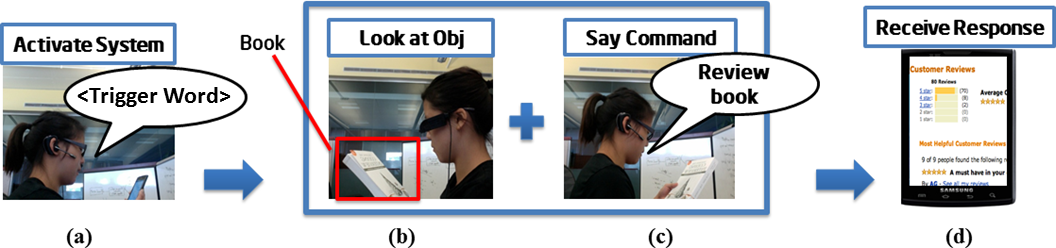
\includegraphics[scale=.45]{fig/poc.png}
%\caption{The MMFPS use case: A person wearing the system (a) gets the system's attention via a trigger word, (b) looks at an object of interest, (c) poses a spoken query about the object, and (d) receives a response on her mobile device.}
%\label{fig:mmfps-usecase}
%\end{figure}
\begin{figure}[t]
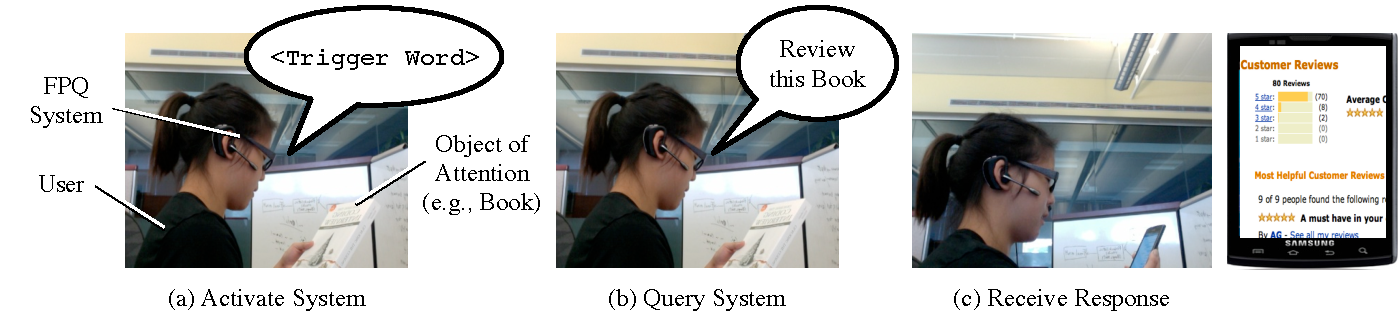
\includegraphics[width=\linewidth]{fig/FPQ.pdf}
\caption{The FPQ use case: A person wearing the system (a) activates the system via a trigger word, (b) makes a verbal query about the object, and (c) receives a response on her mobile device.}
\label{fig:mmfps-usecase}
\end{figure}
The usage scenario for the FPQ system is as follows (see Figure~\ref{fig:mmfps-usecase}): A user wearing a head-mounted camera together with a bluetooth microphone explores the environment by looking at objects and verbally querying the system about objects of interest. For
example, the user may ask ``Where have I seen that person before?'', or ``Can you give me reviews for this item?''. The system sends the requested information to the user's display, such as an android mobile device (see Figure~\ref{fig:mmfps-hardware}). 
\begin{figure}
\centering{
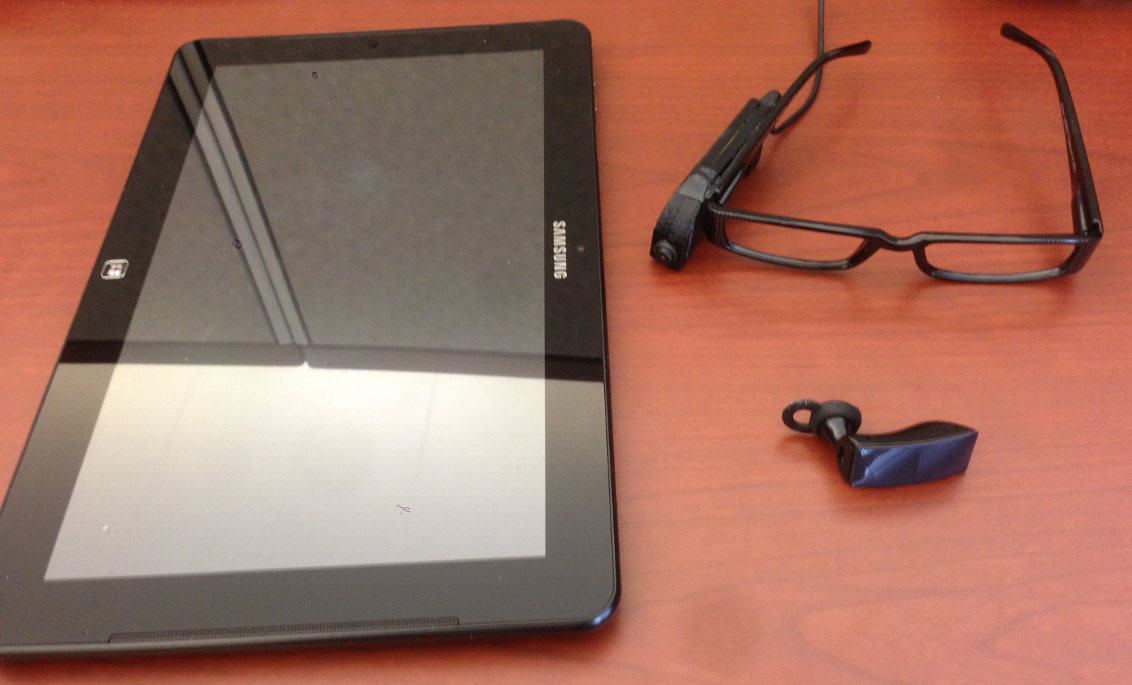
\includegraphics[height=1in]{fig/mmfps_components.jpg}
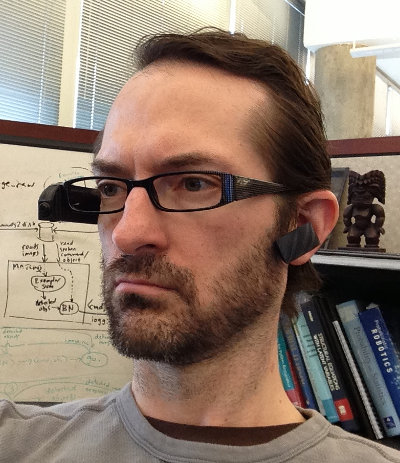
\includegraphics[height=1in]{fig/mmfps_model2.jpg}
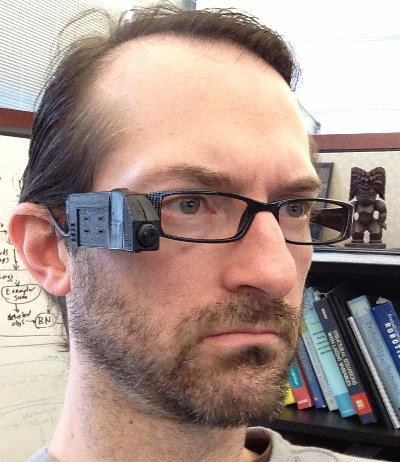
\includegraphics[height=1in]{fig/mmfps_model1.jpg}
}
%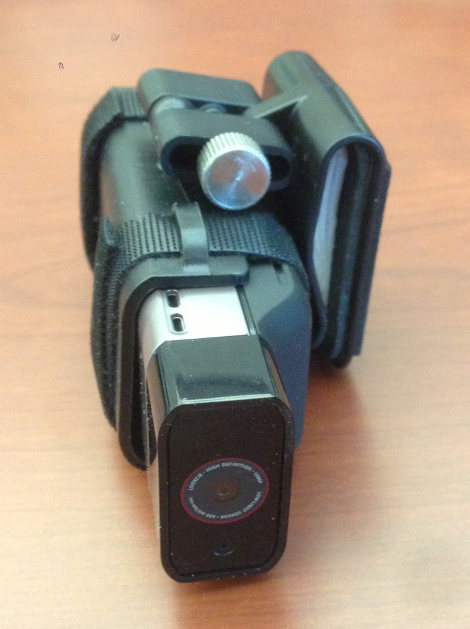
\includegraphics[height=1in]{fig/looxcie.jpg}
\caption{The FPQ hardware components. The system consists of a first person vision camera mounted to an eyeglass frame, an attachable bluetooth microphone, and an android display.}
\label{fig:mmfps-hardware}
\end{figure}

For a system such as this to operate correctly, it must be able to
relate entities being looked at to semantic instances , i.e., it must
perform robust object recognition, which is still an open
problem. However, because this system would be used by a human, there
are other sources of information that can inform the vision subsystem
of the intent of the user. For example:
\begin{enumerate}
\item
\textbf{Trigger Words}. To avoid false positives, the user can issue a trigger keyword to inform the system that he/she is about to pose a query (e.g., ``Jarvis!", or ``Intelligensia!"). 
\item
\textbf{Gaze Direction}. The head pose of the user is strongly correlated with the gaze direction, which is aligned to the object of interest, 
\item
\textbf{Verbal Context}. Commands issued by the user provide cues for the objects of interest. For example the words ``price''  may indicate that the user is referring to a retail object. 
\item
\textbf{Verbal Query}. The user can explicitly refer to object attributes to assist the vision subsystem. For example, the user may say ``where did I meet that brunette Asian girl with glasses?''.
\end{enumerate}
%% In order to facilitate this use-case, the following system components
%% and software packages were used in the MMFPS system:
%% \begin{description}
%% \item [Speech Recognition:] PocketSphinx  \citep{pocketsphinx},
%% \item [Object Instance Recognition:]  The {\em Exemplar-SVM} algorithm and code of \citet{exemplarsvm}, 
%% \item [Face Detection and Recognition:]  The algorithms of \citet{Viola01robustreal-time,fisherfaces} and 
%%   \citet{lbph} based on the implementations in OpenCV \citep{opencv},
%% \item [Visual location recognition:] The 3d reconstruction algorithm of \citet{3dreconstruction}, 
%% \item  [Bayesian Network Classifiers] The SMILE library of \citet{smile}, and
%% \item [System architecture:] The Robotic Operating System (ROS) of \citet{ros} .
%% \end{description}
In Section~\ref{sec:system_arch}, we describe in detail the
architecture design of the FPQ system that brings these various
components together.

\section{System Architecture Design}
\begin{figure} [t]
\centering{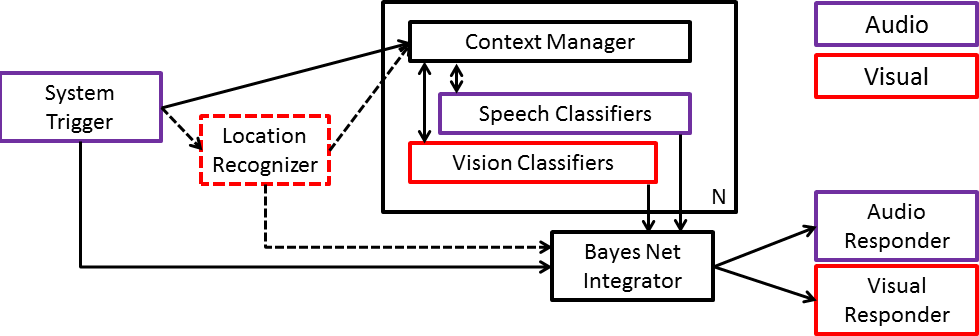
\includegraphics[scale=.4]{fig/system_overview.png}}
\caption{FPQ System Architecture. The purple boxes refer to audio-based components and the red boxes refer to vision-based components.}
\label{fig:system_arch}
\end{figure}
\label{sec:system_arch}
Figure~\ref{fig:system_arch} shows the high-level architecture design of the FPQ system.  The purple boxes indicate audio-based components and the red boxes indicate vision-based components. 
%A speech-based trigger word is used to activate the system, which may then trigger an optional location recognizer. If the location component is present in the system, it
%estimates location and simultaneously informs the context nodes of location and triggers them to activate. If the location node is not present, the context nodes are triggered directly by the System Trigger node.
The system is able to reason about $N$ types of unknown context (e.g.,
the $\langle \texttt{command, object}\rangle$ pair is the ultimate
context to be determined, but there are other auxiliary contexts such
as \texttt{object color} or \texttt{person gender}), each of which can
be detected by a collection of speech or vision-based classifiers.
Each context type possesses a single {\em Context Module} which
consists of a {\em Context Manager}, a list of {\em Speech
  Classifiers} and a list of {\em Vision Classifiers}.  The Context
Manager is a singleton header class which manages all the data related
to its context, which may be location dependent, and activates the
classifiers with the appropriate context data.  It contains methods to
add, delete, update data entries in the library, and will inform other
parts to reload data once modifications in the module data library are
detected. It makes sure that all classifiers in the module share the
same up-to-date data. XML is adopted as the primary data repository
format. Each Context Module has a different set of data for different
scenarios, but with similar formats.

All system classifiers operate in parallel, and the outputs of the classifiers are relayed to the {\em Bayesian Network Integrator} (or just {\em Integrator}) node, which determines the most likely $\langle \texttt{command, object}\rangle$ pair, and forwards that information to an {\em Audio Responder} node and a {\em Visual Responder} node, which respond to the user via verbal or visual feedback.  The Integrator Node can operate asynchronously, providing the best response based on whatever evidence it has received so far until it receives a new system trigger. In the remaining sections, we explain in more detail how our Speech, Vision and Integration subsystems work.

\subsection{Speech Dialog Subsystem}
A speech-based classifier is a pair
$\langle{\cal{S}}(A;D,L),{\cal{M}}(S;D,C)\rangle$, where $\cal{S}$ is a
speech recognition system and $\cal{M}$ is a mapping from sentences to
semantic concepts $C$.  The speech recognition system ${\cal{S}}(A;D,L)$
takes as input a dictionary of words $D$, a language model $L$
specifying how words can be ordered in sentences, and an audio stream
$A$. It outputs a recovered sentence $S$ which is an ordered tuple of
words from $D$. The mapper ${\cal{M}}(S;D,C)$ takes the dictionary $D$, a
set of concepts $C$, and a sentence $S$ as input and outputs a concept
$c\in C$.  We used the speech recognition engine
PocketSphinx \citep{pocketsphinx} in our implementation.

The set $C$ defines what type of concepts the classifier is trying to
identify, and it typically includes a special concept we denote as
\texttt{NA} indicating only that none of the other concepts were
present. As an example, a speech classifier for recognizing gender
might have a dictionary $D$ that included the words $\{\texttt{man,
  boy, woman, girl}\}$ and might have a concept set $C=\{\texttt{male,
  female,\mbox{ NA}}\}$. In our instantiation, the mapper $\cal{M}$
is a bag-of-words model that ignores the order of words in a sentence
and bases its output on which words appear in the sentence compared to
a labeled training set of utterances. 

The System Trigger is a special speech-based classifier in our
implementation that is used to prompt all the Context Modules into
action. As such, it is important to minimize false positives for this
particular classifier.  We accomplish this using the following scheme:
First, we pick a distinctive trigger word. Second, we use an {\em
  open} language model where there are essentially no constraints in
how words appear, and third, we use a relatively large (4000) word
dictionary. For other non-trigger speech-based classifiers, we use a
much smaller dictionary of words and a {\em closed} or more
constrained language model constructed from data of positive instances
of people querying within the context of interest.

%% \subsubsection{Language Analysis}

%% There are two components in a desirable semantic command, the verb and the noun. For example, “recognize this person” is clear to the system, what the user wants from it. Given a sentence, it is relatively straightforward to check which noun appears in the command, while for verbs, it becomes a little tricky. In our design, we used a simple bag-of-words classifier from prior trained data. For example, in the sentence “how do people like this book”, the keyword “like” indicates that the user wants to know the review about this book. In cases when more than one verb keyword are recognized, past queries are referred to determine the actual command.

%% \subsubsection{Adaptation}

%% Four types of adaptation are defined, as indicated in table 1 \citep{niklfeld2001}. Among them, user-controlled user adaptation and system-controlled situation adaptation are adopted in this speech system. To put it easily, system-controlled situation adaptation means that, the system determines which scenario the user is using the system in, without any explicit indication from the users. Similarly, user-controlled user adaptation means that, the user explicit indicates the system his personal habits, allowing solid user adaptivity for the system.

%% {\footnotesize
%% \begin{table}
%%     \begin{tabular}{|l|l|l|}
%%         \hline
%%         ~              & {\bf Situation attributes}                   & {\bf User attributes}                   \\ \hline
%%         {\bf User control}   & User-controller situation adaptation  & User-controlled user adaptation \\  \hline
%%         {\bf System Control} & System-controlled situation adaptation\, & System-controlled user adaptation\, \\ \hline
%%     \end{tabular}
%% \label{tab:adaptation}
%% \caption{Four types of adaptation.}
%% \end{table}
%% } To be more specific, a full-size vocabulary is fed to all speech
%% recognizers, while language models differs between each

%% other. Whenever the user issues a command, all recognizers try to
%% understand the command, and, in most cases, only one of the
%% recognizers is able to get reasonable results. The system figures out
%% the situation of the user based on this result, so this is called
%% system-controlled situation adaption. For user-controlled user
%% adaptation, the user explicitly commands the speech engine to add or
%% delete one data entry to the system repository, so that other
%% recognizers can realize the update in the database to adapt themselves
%% to the user. This feature makes more sense in the multi-modal context
%% than in the speech-alone context.

\subsection{Vision Subsystem}
A vision-based classifier ${\cal V}(F;C)$ takes as input an image
frame $F$ and outputs an indicator $I\in\{\texttt{true, false}\}$
indicating whether a given context $C$ was recognized in the
image. Which algorithms are required for these classifiers depend
strongly on the context being recognized.  Here we detail the
algorithms which we have implemented for various contexts.

\subsubsection{Object Detection}
We use the Exemplar SVM algorithm and code of \citet{exemplarsvm}.  The training
process of Exemplar SVM aims at learning a large-margin decision
boundary between positive and negative samples using only one positive
instance and a large collection of negative samples. At run time, the
Exemplar SVM classifier performs a sliding window scan of an image and
a pyramid search over scales to find the maximum response of a HOG
filter trained on a single view of the target object. We use a C++ version of the real-time recognition portion of the Matlab code
used by \citet{exemplarsvm}.

%% Since the non-parametric nature during
%% testing, it is convenient for us to do meta-information transfer
%% (e.g. semantic segmentation, geometric information) from our training
%% samples to testing images. In the current system, 12 objects were
%% trained, including objects from a retail scenario.
%% \subsubsection{Offline Training}
%% In the offline training stage, each model is learned by optimizing a
%% single-positive-instance SVM problem. Each positive instance is a
%% rigid HOG template of the image patch drawn according to ground-truth
%% bounding box. Following what \citet{exemplarsvm} describes
%% in their training process, we let each exemplar define its own
%% template size. Negative samples are image patches of the same size as
%% positive template drawn from random images on the Internet. Since the
%% decision boundary in Exemplar SVM is largely determined by negative
%% samples instead of the positive sample, the hard-negative mining
%% strategy is employed to do SVM training among large collection of
%% negative samples \citet{lsvm-pami}.

%% \subsubsection{Online Testing}
%% During testing phase, all exemplars are tested on the testing image in
%% a sliding-window fashion. After extracting HOG feature of an testing
%% image, the online testing of an Exemplar SVM on an image patch is just
%% a multiplication operation between the learned template and the HOG
%% feature of that patch. A threshold is set to define ``firing" of a
%% template on an image patch. For all fired bounding boxes, which
%% contains target image patch, non-maximum suppression is then applied
%% to generate a sparse set of detections per image.

\subsubsection{Face-based Classification}
For visual detection of person attributes such as face recognition as well as age, gender, emotion, etc, we employ both the Local Binary Patterns Histograms (LBPH) algorithm
of \citet{lbph} and the ``Fisherfaces'' algorithm of \citet{fisherfaces}, together with training data specific to the attribute at hand. Our implementations of these algorithms are based
on the OpenCV implementations \citep{opencv}. The pipeline for classifying face-based features is shown in
Figure~\ref{fig:face_classifiers}.
\begin{figure}[t]
\centering{  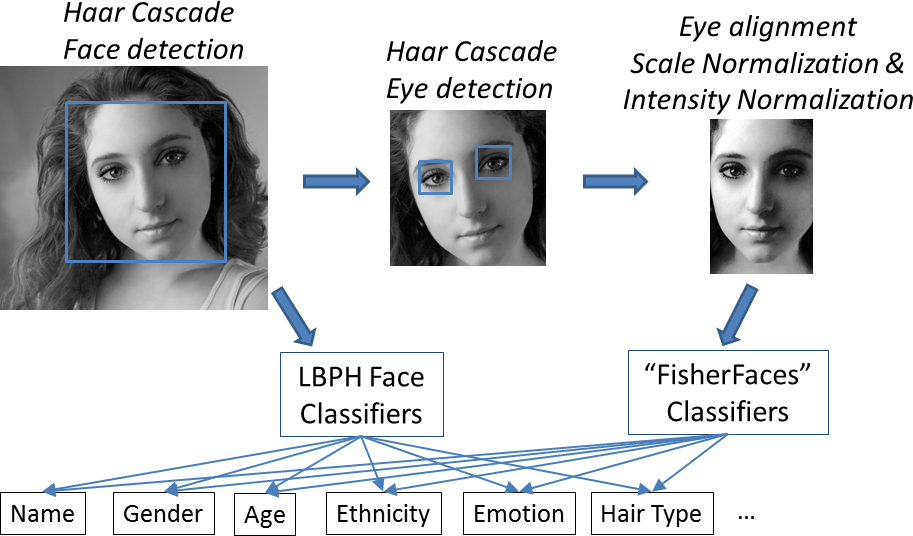
\includegraphics[scale=.4]{fig/face_classifiers.png}}
\caption{The face-based classification pipeline.}
\label{fig:face_classifiers}
\end{figure}
The LBPH classifier has the advantage of not requiring faces to be
aligned or normalized either in intensity or scale. Therefore, LBPH
will give results in some cases where FisherFaces will not. In order
to use these algorithms for face attribute classification, training
data is partitioned according to the attribute of interest. For
example, a gender detector was built by training on data that has been
partitioned into male and female subsets.

Breaking faces (or objects in general) up into attributes serves two
important purposes for our system. First, describing a face as a
feature vector of attributes culled from face images has been shown to
improve face recognition significantly by
\citet{Kumar09attributeand}. Second, these attributes provide
``hooks'' by which users can collaborate with the vision subsystem by
specifying attributes of interest.

\subsection{Integration Engine}
The integration engine collects the outputs of all classifiers and
makes a global decision about the most likely $\langle
\texttt{command, object}\rangle$ pair. We use a Bayesian network
to accomplish this task, the structure of which  will depend on
which bits of context are being monitored by the system and on how
elaborate we choose to make the model. One example of a model
that makes use of multiple face-based attribute detectors, location,
and both textured and untextured object detectors is shown in
Figure~\ref{fig:bn_full}.
\begin{figure} [t]
\centering{  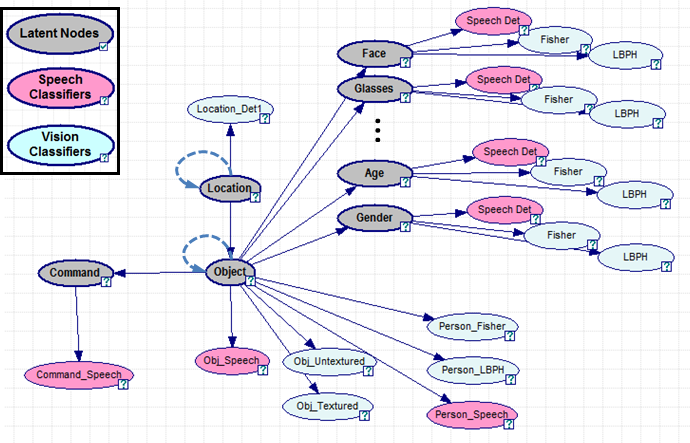
\includegraphics[scale=.5]{fig/bn_full.png}}
\caption{An expansive Bayesian network model that includes all the components in our designed system.}
\label{fig:bn_full}
%centering{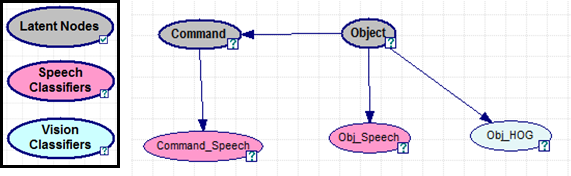
\includegraphics[scale=.55]{fig/bn_poc.png}}
%\caption{The Bayesian network model used for our first proof-of-concept.}
%\label{fig:bn_poc}
\end{figure}
In this figure, gray nodes indicate latent context variables which we
would like to infer from the classifier outputs. Pink nodes indicate
observed speech classifier output variables, and light blue nodes
indicate observed vision-classifier variables.

The set of likely commands depend on the object of interest. Thus the
model has an arc from $\texttt{object}\rightarrow \texttt{command}$, with a conditional
probability table (CPT) indicating this asymmetry. For a given object,
we assume that all commands which apply to that object are equally
likely, although the CPT could easily be adapted to learn an
empirical prior. Similarly, if \texttt{location} is
included (e.g., via GPS or visual localization) in the model, as in Figure~\ref{fig:bn_full}, then the \texttt{object} node possesses a CPT which reflects asymmetry in how
objects/people are likely to be distributed in space. This
Location-dependent list of objects would be especially useful in
structured environments such as retail establishments, and could
assist as a prior in scaling up classifier algorithms that may not scale well
with the number of objects.

The CPT of a classifier node summarizes the confusion matrix of the
classifier, i.e., the CPT entry $\theta_{ij}$ specifies the
probability that the classifier will output the context label
$\hat{c}_i$ given that the actual label was $c_j$:
$\theta_{ij}=P(\hat{C}=\hat{c}_i|C=c_j)$.  These probabilities are
estimated from labeled training data. There will exist
some context states $c_i$ which do not have a corresponding classifier
label so will not be present in the training data.  For example a face
recognizer classifier will not have a label for a retail object. To
handle these cases and to produce smooth CPTs, we assume Laplacian
priors during the CPT learning process, which typically results in
weak uniform priors for the portion of the CPT corresponding to
unrepresented context states in the classifier output symbols. 

It is straightforward to incorporate temporal smoothness by converting this static
Bayesian network into a dynamic Bayesian network. In
Figure~\ref{fig:bn_full}, we have drawn dashed self-edges to $\texttt{location}$
indicating a motion model, and to $\texttt{object}$ indicating the fact that a
user can switch object of interest over time without having switched
location.

\section{Instantiation and Testing}
We instantiated a version of our architecture design with three
classifiers: a speech-based command recognizer, a speech-based object
recognizer, and a vision-based untextured object recognizer.  The
Bayesian network model for this case is shown in
Figure~\ref{fig:bn_poc}.
\begin{figure}
\centering{  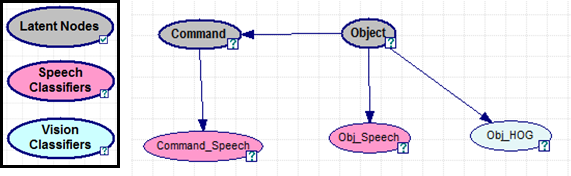
\includegraphics[scale=.5]{fig/bn_poc.png}}
\caption{The integrator model used for the performance test.}
\label{fig:bn_poc}
\end{figure}


The Exemplar SVM was trained on 150 images containing 12 object
classes. The objects used are shown in Figure~\ref{fig:test_objects},
in which 15 objects are present. Some objects were combined into the
same object class resulting in 12 classes total. Training data was
collected by 10 hours of use in a cluttered environment(see
Figure~\ref{fig:test_objects}) with YouTube videos playing in the
background to simulate a noisy environment. The overall accuracy of
the Exemplar SVM algorithm on this data was measured to be $P_v
=74\%$.
\begin{figure}
\centering{  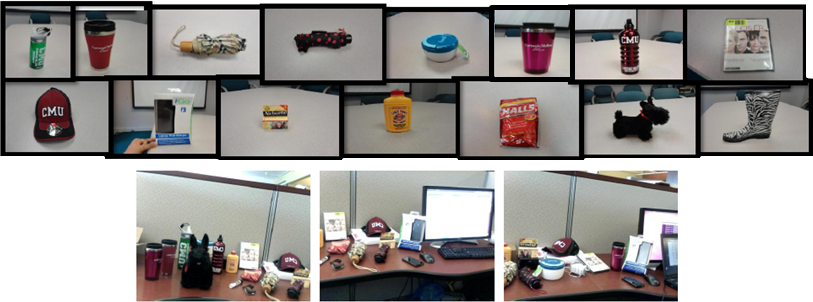
\includegraphics[scale=.5]{fig/test_objects.png}}
\caption{The 15 objects used for the performance tests and some
  examples of cluttered scenes used for the test.}
\label{fig:test_objects}
\end{figure}

We used three commands for querying: ``Information'', ``Option'' and
``Review'', and the average speech recognition accuracy was $P_s =
86\%$. Using our Integrator model, the probability of recovering the
correct $\langle \texttt{command, object}\rangle$ pair was
$P_{sys}=88.4\%$. On the other hand, if we were to treat the speech
and vision components independently and take the command from the
speech classifier and the object from the vision classifier, we would
have a joint accuracy of:
\begin{math}
P_{ind} = 1 - \{(1-P_s)* P_{v} + P_s * (1-P_v) + (1-P_s)\cdot (1-P_v)\} = 0.63,
\end{math}
implying an improvement of the joint $\langle \texttt{command,
  object}\rangle$ of nearly $40\%$ with our system.  This case does
not yet make use of the $\texttt{object}\rightarrow \texttt{command}$
arc since all objects had the same set of commands, nor does it make
full use of the human collaborative aspect because there were no
object attribute classifiers included in the model. While these
results are reported based on an initial test case, they are
encouraging and indicate that this approach has the potential to
dramatically improve perception accuracy on a more complex model.


\section{Discussion}
We have presented a multi-modal first-person system---i.e., a system
that sees what the user sees and hears what the user says---to allow
users to verbally query and visually receive information about objects
and people in their physical environment. We have discussed the
complete system architecture design, which analyzes video and audio
acquired from the user's perspective, integrates multiple classifiers
via a graphical model, and in real-time infers the the user's query
and object of interest, providing seamless interaction between the
user and the environment. Our first instantiation of the system design
shows that by combining multiple modalities and multiple classifiers,
our method improves inference accuracy of the joint
$\langle$\texttt{command, object}$\rangle$ pair by $39\%$ over a
system that treats the spoken command and the visual object
recognition inference problems independently.

Our next steps would be to expand our instantiation of the system to
include a wider range of modular components as outlined in our design,
and to incorporate automated semi-supervised updating of parameters in
real time. We plan to integrate vision-based localization (e.g., as in
\citep{Park12}) to provide 3D location context to the system. We will
also investigate ways to integrate first-person displays for user feedback.

%\subsubsection{Textured Objects}
%For textured objects, we plan to use the MOPED library of
%\citet{moped}. The MOPED algorithm builds detailed 3d models of highly
%textured objects in an offline training phase that uses structure from
%motion to establish a map of SIFT features for each object. In
%real-time these models are used by matching SIFT features in a given
%frame to those of the models, and by simultaneously aligning SIFT
%features and refining the matches by applying multiple RANSAC
%iterations. \citeauthor{moped} have published ROS versions of the
%MOPED library.
%

%\subsubsection{Location}
%For indoor location determination, we employ the algorithm and code
%from \citet{Park-12} which uses structure from motion to
%perform an offline 3d reconstruction of the SIFT point cloud of a
%physical environment. Once such a point-cloud is constructed and
%mapped to physical locations in the space of interest, it can be used
%for precise ($\sim \pm 1m$) real-time vision-based localization by
%matching SIFT features in a given frame to the reference point-cloud.
%
% ---- Bibliography ----
%
\footnotesize
\bibliographystyle{plainnat}
\bibliography{mmfps}
\end{document}

